\section{Решение проблемы}
\label{sec:Chapter2} \index{Chapter2}

В настоящей работе исследуется возможность ускорения расчета плотности атмосферы c
использованием интерполяционных подходов.

Существует несколько хорошо известных алгоритмов многомерной интерполяции. Полилинейная и
поликубическая интерполяция, а также интерполяция до ближайшего характеризуются низкой
вычислительной сложностью, но малой точностью. 
Компромиссом является интерполяция на узлах Чебышева--Лиссажу \cite{dencker2017}, обеспечивающая
быструю многомерную интерполяцию с сохранением высокой точности. 
Именно этот алгоритм был выбран для интерполяции модели атмосферы.

\subsection{Обзор алгоритма интерполяции}
Первый этап создания интерполянта на узлах Чебышева--Лиссажу заключается в построении 
прямоугольной сетки в $\mathbb{R}^d$. В частном случае это сетка в
околоземном пространстве в координатах $(r, \phi, \lambda, t)$.

Затем для ячейки сетки вычисляется набор точек, являющихся обобщением
узлов Чебышева--Гаусса--Лобатто на $d$--мерное пространство:

\begin{equation*}
    \begin{cases*}
        \mathbf{z_{\mathbf{i}}^{\mathbf{(\mathbf{n})}}} = (z_{i_1}^{n_1}, \dots, z_{i_d}^{n_d}) \\
        z_i^{n} = \cos (i \pi / n)
    \end{cases*}
\end{equation*}

Наборы $\mathbf{i} \in \mathbb{N}^d$ состоят либо лишь из четных, либо только из нечетных чисел, при этом каждое
число не превышает соответствующее число из $\mathbf{n} \in \mathbb{N}^d$, 
состоящего из взаимно простых чисел и определяющего конфигурацию интерполянта.

Эти узлы лежат в точках самопересечения кривых Лиссажу:

\begin{equation*}
    \mathbf{l} = \left(\cos \left( \frac{\pi * p[\mathbf{n}]}{n_1} \right), 
                \dots,\cos \left( \frac{\pi * p[\mathbf{n}]}{n_d} \right) \right),
\end{equation*}
где $p[\mathbf{n}] = \prod_{j=1}^{d} n_j$.

Визуализация узлов и кривых Лиссажу для трехмерного пространства представлена на рис. \ref{fig:chebLis}.

\begin{figure}[h!]
    \centering
    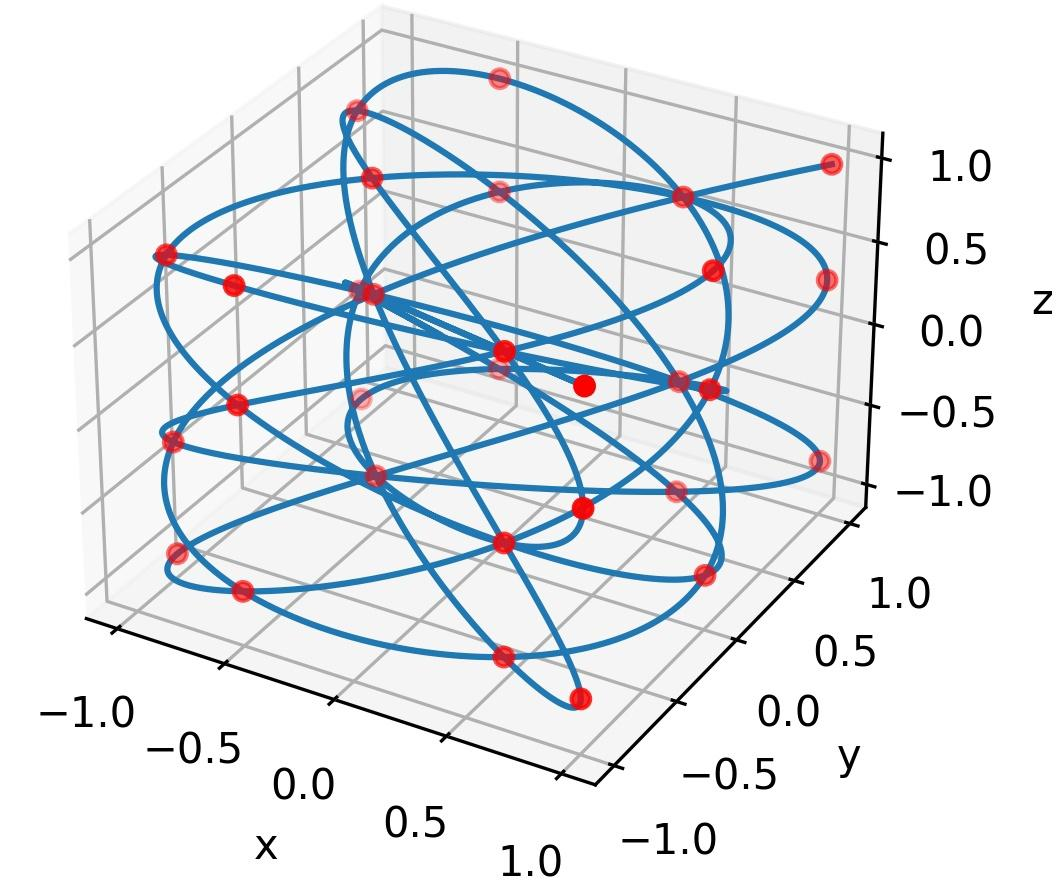
\includegraphics[width=0.5\linewidth]{../images/solution/chebLis.png}
    \captionof{figure}{Узлы Чебышева--Лиссажу в единичном кубе}
    \label{fig:chebLis}
\end{figure}

Теперь необходимо найти d-мерный полином, удовлетворяющий условию интерполяции.

Полиномы Чебышева имеют следующий вид:
\begin{equation*}
    T_{\gamma} (x) = \cos (\gamma \arccos (x))
\end{equation*}

В узлах Чебышева--Лиссажу:
\begin{equation*}
    T_{\gamma} (z^n_i) = \cos \left(\gamma \arccos \left(\cos \left(\frac{i \pi}{n}\right) \right)\right)
     = \cos(\gamma \frac{i \pi}{n}) \equiv \chi_{\gamma}^n (i)
\end{equation*}

Определим d-мерные полиномы Чебышева как:
\begin{equation*}
    T_{\mathbf{\gamma}} = T_{\gamma_1} \cdot \dots \cdot T_{\gamma_d},
\end{equation*}
где $\mathbf{\gamma} \in \mathbb{N}^d_0$.
Они составляют ортогональный базис в d-мерном пространстве полиномов. Аналогично,
\begin{equation*}
    \chi_{\mathbf{\gamma}}^{\mathbf{n}} (\mathbf{i}) = \prod_{j=1}^{d} \cos(\gamma_j \frac{i_j \pi}{n_j})
\end{equation*}
В свою очередь $\chi_{\mathbf{\gamma}}^{\mathbf{n}} (\mathbf{i})$ составляют базис в пространстве
функций $L^2$.

Этот факт дает возможность разложить, функцию $h$, заданную на узлах, по данному базису, чтобы
получить коэффициенты интерполяции:
\begin{equation*}
    \begin{cases*}
        h \approx \sum_{\mathbf{\gamma}} c_{\mathbf{\gamma}} (h) \chi_{\mathbf{\gamma}}^{\mathbf{n}} \\
        c_{\mathbf{\gamma}} (h) = \frac{1}{|| \chi_{\mathbf{\gamma}}^{\mathbf{n}} ||^2}
        \left(h, \chi_{\mathbf{\gamma}}^{\mathbf{n}}\right)
    \end{cases*}
\end{equation*}

Вид базисных функций позволяет последовательно
применить дискретное косинус преобразование к каждой размерности для эффективного подсчета
коэффициентов. 

В результате функция может быть аппроксимирована линейной комбинацией произведений
многочленов Чебышева:
\begin{equation*}
    h \approx \sum_{\mathbf{\gamma}} c_{\gamma} T_\gamma
\end{equation*}

В частном случае интерполяции 4-мерной функции плотности атмосферы
результат интерполяции представим в виде:
\begin{equation*}
    \ln(\rho) \approx \sum_{i,j,k,l}^{n_1, n_2, n_3, n_4} 
    c_{i,j,k,l} T_i(r) T_j(\phi) T_k (\lambda) T_l (t),
\end{equation*}
где $T_\alpha$ -- полином Чебышева степени $\alpha$.

Интерполяция логарифма объяснятся тем фактом, что зависимость убывания
атмосферной плотности с высотой примерно экспоненциальная.

Точность интерполяции определяется количеством ячеек, на которое было разбито пространство
и максимальной степенью полиномов по размерности для каждой ячейки.

Скорость интерполяции зависит от конфигурации интерполянта. Чем больше степени полиномов в
каждой ячейке, тем сильнее увеличивается время подсчета.
\newpage